% Abstract file structure example : 
% \abstitle{title here}
% \absauthors{names and superscripts for affiliations here}
% \absaddress{affiliations, starting each one with its superscripts, separate affiliations with a \break}
% \abstext{
% \index{author abbreviated name, to be placed in authors' index}
% \index{create an index entry for each author}
%  The abstract text
% }

%% Abstract title
%\abstitle{Studio sui chirotteri troglofili della Grotta di Calafarina (Pachino, SR, Sicilia sud-orientale)}

%% Author names
%\absauthors{M. \textsc{Mucedda}$^1$,  G. \textsc{Fichera}$^2$, E. \textsc{Pidinchedda}$^1$}

%\absaddress{$^1$Centro Pipistrelli Sardegna, Via G. Leopardi 1 – 07100 Sassari, Italy - batsar@tiscali.it\break
%$^2$Universität Trier Universitätsring,15 - D-54286  Trier, Germany}

%% Abstract text
%\abstext{
%%% Author names for index. State each author separately using \index{Doe J.}
%\index{Mucedda M.}
%\index{Fichera G.}
%\index{Pidinchedda E.}
%%% The actual abstract text goes here
%} %% remember to close the abstract text block brace!!
\label{ext:P001}

\loadabstr[P001]{DE PASQUALE P.P. -- I Chirotteri del Parco Nazionale dell'Appennino Lucano Val d'Agri Lagonegrese}{abstracts/extended_abstracts/P001_depasquale_extended_title.tex}

\begin{multicols}{2}

\section*{Introduzione}
Il Parco Nazionale Appennino Lucano val d’Agri Lagonegrese, è ubicato nell’area appenninica sud-occidentale della Basilicata, ai confini con la Campania (Italia meridionale). L’area protetta si estende per circa 69000 ettari ed è caratterizzata prevalentemente da un paesaggio montuoso molto complesso ed eterogeneo, intervallato da ampie vallate, con rilievi che giungono a circa 2000 m di altitudine (Monte del Papa, 2005 m s.l.m.). Esso rappresenta il secondo Parco Nazionale lucano e insieme al Pollino protegge circa il 16\% della superficie regionale. Il comprensorio del Parco è rappresentato da zone a clima spiccatamente temperato e le aree dislocate a media e bassa quota risentono di un clima di carattere mediterraneo. Il presente lavoro descrive le conoscenze acquisite da luglio a settembre 2012, relative al  primo studio sulla chirotterofauna del Parco. Gli obiettivi del lavoro sono: compilare una \textit{checklist}, effettuare un censimento preliminare dei rifugi utilizzati, della distribuzione potenziale e delle relazioni specie-habitat, attraverso la progettazione di modelli d’idoneità ambientale specie-specifici.

\begin{table*}[t]
\caption*{Tab. 1 - Checklist della chirotterofauna censita nel Parco Nazionale dell’Appennino Lucano.}
%\label{tab:table1}
\centering\small
\begin{tabular}{llcc}
\textbf{Famiglia}&\textbf{Specie}&\textbf{Lista Rossa Nazionale}&\textbf{Direttiva Habitat}\\
\hline
VESPERTILIONIDAE & \emph{Pipistrellus  kuhlii} & Rischio minimo (LC) & IV \\
VESPERTILIONIDAE & \emph{Pipistrellus pipistrellus} & Rischio minimo (LC) & IV \\
VESPERTILIONIDAE & \emph{Pipistrellus pygmaeus} & Dati insufficienti (DD) & IV \\
VESPERTILIONIDAE & \emph{Hypsugo savii} & Rischio minimo (LC) & IV \\
VESPERTILIONIDAE & \emph{Nyctalus leisleri} & Prossima alla minaccia (NT) & IV \\
VESPERTILIONIDAE & \emph{Nyctalus noctula} & Vulnerabile (VU) & IV \\
MOLOSSIDAE & \emph{Tadarida teniotis} & Rischio minimo (LC) & IV \\
RHINOLOPHIDAE & \emph{Rhinolophus ferrumequinum} & Vulnerabile (VU) & II, IV \\
RHINOLOPHIDAE & \emph{Rhinolophus euryale} & Vulnerabile (VU) & II, IV \\
RHINOLOPHIDAE & \emph{Rhinolophus hipposideros} & Minacciata (EN) & II, IV \\
MINIOPTERIDAE & \emph{Miniopterus schreibersii} & Vulnerabile (VU) & II, IV \\
VESPERTILIONIDAE & \emph{Barbastella barbastellus} & Minacciata (EN) & II, IV \\
VESPERTILIONIDAE & \emph{Myotis myotis} & Vulnerabile (VU) & II, IV \\
VESPERTILIONIDAE & \emph{Myotis daubentonii} & Rischio minimo (LC) & IV \\
VESPERTILIONIDAE & \emph{Myotis nattereri} & Vulnerabile (VU) & IV \\
VESPERTILIONIDAE & \emph{Myotis bechsteinii} & Minacciata (EN) & II, IV \\
VESPERTILIONIDAE & \emph{Myotis alcathoe} & Non valutata &   \\
VESPERTILIONIDAE & \emph{Myotis emarginatus} & Vulnerabile (VU) & II, IV \\
VESPERTILIONIDAE & \emph{Eptesicus serotinus} & Prossima alla minaccia (NT) & IV \\
VESPERTILIONIDAE & \emph{Plecotus austriacus} & Prossima alla minaccia (NT) & IV \\
VESPERTILIONIDAE & \emph{Plecotus auritus} & Prossima alla minaccia (NT) & IV \\
\end{tabular}
\end{table*}

\section*{Materiali e metodi}
L’analisi faunistica si è basata prevalentemente su indagini di campo condotte in taluni casi anche fuori dei confini del Parco, laddove sono stati rilevati \textit{roost} potenzialmente utilizzati. L’approccio metodologico adottato ha considerato le linee guida per il monitoraggio dei chirotteri redatte per l’Italia da Agnelli et al. (2004). La ricerca dei rifugi è stata limitata alla valutazione della presenza di chirotteri solo negli edifici dismessi e nelle cavità ipogee, di origine artificiale (gallerie, condotte sotterranee) e naturale (grotte). Ad oggi, le ricerche speleologiche condotte nell’area di studio hanno rilevato la presenza di un numero esiguo di cavità di origine naturale e non essendo disponibile un catasto regionale delle cavità ipogee, i siti sono stati individuati attraverso la raccolta di dati inediti mediante interviste a speleologi locali e valutando scrupolosamente l’idoneità ambientale di ciascun sito. Le cavità sono state ispezionate nel periodo post-natale e utilizzando luci fredde (LED), mentre il conteggio delle colonie è stato effettuato direttamente da fotografie scattate nel \textit{roost}, e le specie sono state identificate mediante analisi morfometrica o rilievo ultrasonoro all’emergenza serale. Le catture temporanee sono state effettuate nel periodo luglio-agosto 2012, mediante reti del tipo \textit{mistnet} per chirotteri (Ecotone), di 6.0$\times$2.50~m e 12.0$\times$2.50~m e con dimensione di maglia 14 mm (lunghezza di un lato della maglia). Le reti sono state aperte al tramonto per circa 3 ore e monitorate ogni 15 minuti per evitare la mortalità dei chirotteri catturati soprattutto per disidratazione e ipotermia (Kunz e Kurta, 1988). Sono state posizionate per mezzo di paletti telescopici, in prossimità di potenziali aree di foraggiamento, corridoi di volo e zone di abbeverata, come piccoli laghi di montagna, fiumi e torrenti. Nella fase successiva alla cattura, gli individui sono stati riposti in un sacchetto in cotone e poi pesati, mediante bilancia digitale con precisione $\pm$0.1~g, misurati mediante un calibro digitale autobloccante, con precisione $\pm$0.1 mm e poi rilasciati. Inoltre, per ciascun esemplare catturato è stato rilevato il sesso, la classe di età, lo stato riproduttivo. Gran parte delle specie catturate sono state identificate mediante analisi morfometrica e utilizzando le chiavi analitiche di Dietz e Von Helversen (2004). Gli individui appartenenti a \textit{taxon} criptici (\emph{Myotis mystacinus} group), sono stati sottoposti a una biopsia della pelle (\textit{biopsy punch}); il materiale biologico è stato estratto mediante un \textit{punch} avente 3~mm di diametro, direttamente dalla membrana caudale (uropatagio) e conservato in provette con etanolo assoluto e in frigorifero (Worthington-Wilmer et al., 1996). I campioni sono stati analizzati attraverso il metodo del DNA Barcoding (Hebert et al., 2003; Galimberti et al., 2012) e identificati geneticamente presso lo ZooPlantLab del Dipartimento di Biotecnologie e Bioscienze dell’Università degli Studi di Milano-Bicocca.

\begin{center}
\captionof*{table}{Tab. 2 - Metodi di indagine per ogni specie rilevata.}
%\label{tab:table1}
\centering\small
\begin{tabular}{lccc}
\textbf{Specie}&
\rotatebox{90}{\textbf{\shortstack[l]{Rilievo\\ultrasonoro}}}&
\rotatebox{90}{\textbf{\shortstack[l]{Cattura\\temporanea}}}&
\rotatebox{90}{\textbf{\shortstack[l]{Analisi\\molecolare}}}\\
% & \textbf{ultrasonoro} & \textbf{temporanea} & \textbf{molecolare} \\
\hline
\emph{Pipistrellus  kuhlii}      &$\times$&$\times$& \\
\emph{Pipistrellus pipistrellus} &$\times$&$\times$& \\
\emph{Pipistrellus pygmaeus}     &$\times$&$\times$& \\
\emph{Hypsugo savii}             &$\times$&$\times$& \\
\emph{Nyctalus leisleri}         &$\times$&$\times$& \\
\emph{Nyctalus noctula}          &$\times$&$\times$& \\
\emph{Tadarida teniotis}         &$\times$& & \\
\emph{Rhinolophus ferrumequinum} &$\times$&$\times$& \\
\emph{Rhinolophus euryale}       &        &$\times$& \\
\emph{Rhinolophus hipposideros}  &$\times$& & \\
\emph{Miniopterus schreibersii}  &$\times$& & \\
\emph{Barbastella barbastellus}  &$\times$&$\times$& \\
\emph{Myotis myotis}             &        &$\times$& \\
\emph{Myotis daubentonii}        &        &$\times$& \\
\emph{Myotis nattereri}          &        &$\times$& \\
\emph{Myotis bechsteinii}        &        &$\times$& \\
\emph{Myotis alcathoe}&        &$\times$&$\times$\\
\emph{Myotis emarginatus}&$\times$&$\times$& \\
\emph{Eptesicus serotinus}&$\times$& & \\
\emph{Plecotus austriacus}&        &$\times$& \\
\emph{Plecotus auritus}&        &$\times$& \\
\end{tabular}
\end{center}

\subsection*{Campionamento bioacustico e analisi dei dati}
Il protocollo di ricerca utilizzato ha previsto anche un campionamento bioacustico stratificato rispetto alla disponibilità ambientale, per punti d’ascolto selezionati in modo \textit{random} in ciascun habitat. Sono stati selezionati 140 punti di ascolto con un tempo di campionamento di 15 minuti per ogni punto. Le unità di campionamento sono state selezionate in un \textit{range} altitudinale di 349--1607 m s.l.m. (min--max). Il picco massimo di attività dei chirotteri, generalmente si rileva nelle prime ore della notte (Gaisler, 1979; Erkert, 1982), per cui il tempo di campionamento per ogni notte è stato di 4 ore, a cominciare da 30 minuti dopo il tramonto ed è stato effettuato solo durante le notti con temperature superiori a \SI{10}{\degree\celsius}, senza precipitazioni e vento (Grindal et al., 1992).

I rilievi ultrasonori sono stati effettuati con un \textit{bat detector} modello Pettersson D 240X, con espansione temporale (10$\times$). I singoli campioni sono stati registrati con un registratore digitale Edirol R-09, con frequenza di campionamento a 44.1~kHz e risoluzione a 16~bit.

L’analisi spettrale è stata effettuata per mezzo del \textit{software} BatSound v. 3.3 (Pettersson elektronik AB, Uppsala, Sweden), utilizzando una frequenza di campionamento di 44.1~kHz e risoluzione a 16~bit e una FFT (\textit{Fast Fourier Transform}) con finestra di Hamming di dimensioni pari a 512 punti/campione, applicando criteri quantitativi per l’identificazione (Russo e Jones, 2002). I parametri spettrali misurati sono i seguenti: frequenza iniziale (SF), frequenza finale (EF), frequenza di massima energia (FMAX), \textit{interpulse interval} (IPI), durata (D). L’identificazione specifica è stata effettuata solo per i \textit{taxa} facilmente riconoscibili e non caratterizzati da un’ampia sovrapposizione interspecifica dei parametri spettrali e temporali dei segnali, come ad esempio quelli appartenenti al genere \emph{Myotis}. Le specie \emph{P. pipistrellus} e \emph{P. pygmaeus} sono state identificate misurando la frequenza di massima energia dei segnali di ecolocalizzazione emessi durante l’attività di foraggiamento e al rilascio dopo la cattura (Russo e Jones, 2000). L’attività dei chirotteri è stata quantificata rilevando il numero di passaggi per habitat attraverso il conteggio delle sequenze dei segnali di ecolocalizzazione (Fenton, 1970) e non facendo distinzione tra le sequenze dei segnali di ecolocalizzazione relative all’attività di foraggiamento, caratterizzate da una serie rapida di segnali (\emph{feeding buzzes}) (Griffin et al., 1960), e le sequenze identificate da due o più pulsazioni consecutive emesse durante gli spostamenti in volo o per la ricerca della preda (Thomas 1988).

\begin{table*}[t]
\captionof*{table}{Tab. 3 - Media, deviazione standard (DS) e min--max del numero di passaggi, per habitat. CER = Cerrete; BOS = Boschi misti di latifoglie; URB = Aree urbane; UMI = Aree umide; RIM = Rimboschimenti a conifere; PRA = Praterie; LEC = Querceti a leccio; FAG = Faggete; COL = Coltivi.}
%\label{tab:table1}
\centering\small
\begin{tabular}{lccccccccc}
 & \multicolumn{9}{c}{\textbf{Habitat}}\\
 & \textbf{CER} & \textbf{BOS} & \textbf{URB} & \textbf{UMI} & \textbf{RIM} & \textbf{PRA} & \textbf{LEC} & \textbf{FAG} & \textbf{COL} \\
\hline
\textbf{Media$\pm$DS}&6.30$\pm$4.60&5.97$\pm$4.66&13.0$\pm$4.24&26.67$\pm$7.02&3.60$\pm$2.61&3.80$\pm$3.36&6.25$\pm$3.50&10.40$\pm$5.41&2.53$\pm$2.01\\
\textbf{min--max}&0--14&0--14&10--16&20--34&0--7&0--10&2--10&1--18&0--6\\
\end{tabular}
\end{table*}

\begin{center}
\captionof*{table}{Tab. 4 - Risultanze del test \textit{post-hoc} di Tukey-Kramer, intervalli di confidenza al 95\% e \prob{}-value per coppie di habitat.}
%\label{tab:table1}
\centering\small
\begin{tabular}{lcc}
\textbf{Habitat}& \textbf{IC 95\%} & \textbf{\prob{}-value} \\
\hline
\shortstack[l]{Cerrete--\\aree umide}&(0.054; 3.147)&0.037\\
\shortstack[l]{Boschi misti di latifoglie--\\aree umide}&(0.096; 3,235)&0.029\\
\shortstack[l]{Rimboschimenti a conifere--\\aree umide}&(-3.866; -0.075)&0.035\\
\shortstack[l]{Praterie--\\aree umide}&(-3.652; -0.369)&0.005\\
\shortstack[l]{Coltivi--\\aree umide}&(-3.862; -0.637)&0.001\\
\shortstack[l]{Faggete--\\praterie}&(0.036; 1.932)&0.036\\
\shortstack[l]{Faggete--\\coltivi}&(-2.120; -0.326)&0.001\\
\end{tabular}
\end{center}

\begin{table*}[t]
\captionof*{table}{Tab. 5 - Rifugi censiti nel territorio del Parco Nazionale dell’Appennino Lucano. R.f. = \emph{Rhinolophus ferrumequinum}; R.e. = \emph{Rhinolophus euryale}; R.h. = \emph{Rhinolophus hipposideros}; M.sch. = \emph{Miniopterus schreibersii}; M.e. = \emph{Myotis emarginatus}}
%\label{tab:table1}
\centering\small
\begin{tabular}{p{25mm}p{30mm}llp{30mm}cp{15mm}}
\textbf{Rifugio} & \textbf{Località} & \textbf{Tipologia} & \textbf{Specie} & \textbf{Ruolo biologico} & \textbf{Abbondanza} & \textbf{Note} \\
\hline
Grotta di Sant’Angelo al Raparo & San Chirico Raparo (PZ) &	Cavità naturale &	R.e. & riproduzione, svernamento & 2000 & \\	
& & & R.f. & riproduzione, svernamento & 200	 & \\
& & & R.h. & rifugio  temporaneo & n.d. & \\	
& & & M.sch. & rifugio  temporaneo & n.d. \\
Grotta Murgia Sant’Angelo & Moliterno (PZ) & Cavità naturale & R.e. & riproduzione & 800 & \\	
& & & M.sch. & rifugio temporaneo & 1 & \\	
Grotta dell’Aquila & Tramutola (PZ) & Cavità naturale & R.h. & n.d. & n.d. & \\
Galleria FCL & Pignola (PZ) & Cavità artificiale & R.f. & svernamento e altra funzione non accertata & n.d. & \\
Grotta di Castel di Lepre & Marsico Nuovo (PZ) & Cavità naturale & R.f. & n.d. & 10 & \\
Edificio Trifolco & San Martino d’Agri (PZ) & Edificio & R.e. & rifugio temporaneo & 8 & \\	
Edificio & Moliterno (PZ) & - & R.h. & rifugio temporaneo & 3 & \\	
Masseria dei Romani & San Martino d’Agri (PZ) & Edificio & R.e. & rifugio temporaneo & 3 & \\	
Gavitedde (edificio 1) & San Martino d’Agri (PZ) & Edificio & R.e., M.e. & rifugio temporaneo & 2 & \\	
Gavitedde (edificio 2) & San Martino d’Agri (PZ) & Edificio & R.f. & rifugio temporaneo & 5 & \\	
Torre San Nicola & Moliterno (PZ) & Edificio & R.f. & rifugio temporaneo & 2 & \\	
Masseria Crovattiera & San Martino d’Agri (PZ) & Edificio & n.d. & n.d. & n.d. & presenza di guano \\
\end{tabular}
\end{table*}

I dati dei conteggi sono stati trattati e sottoposti ad una trasformazione logaritmica, mediante logaritmo naturale, secondo la formula $ln(\text{N passaggi} + 1)$. È stato valutato statisticamente l’effetto del tipo di habitat sull’attività dei chirotteri attraverso un’analisi della varianza (\textit{one way} ANOVA), con livello di significatività \prob{}=0.05, in cui le tipologie ambientali rappresentano la variabile indipendente e il numero di passaggi di chirotteri rappresenta la variabile dipendente. Prima di procedere con l’analisi, è stato applicato il test di Hartley, per verificare l’omogeneità della varianza campionaria. Dopo aver effettuato l’analisi della varianza, per valutare in quali habitat le differenze dell’attività sono significative, è stato applicato il test \textit{post-hoc} HSD di Tukey-Kramer, facendo confronti multipli delle medie tra coppie di habitat, per un numero ineguale di unità campionarie (Tukey, 1949; Kramer, 1956). Le analisi statistiche sono state effettuate mediante il \textit{software} Minitab 17.

\begin{Figure} %[!ht]
  \centering\small
  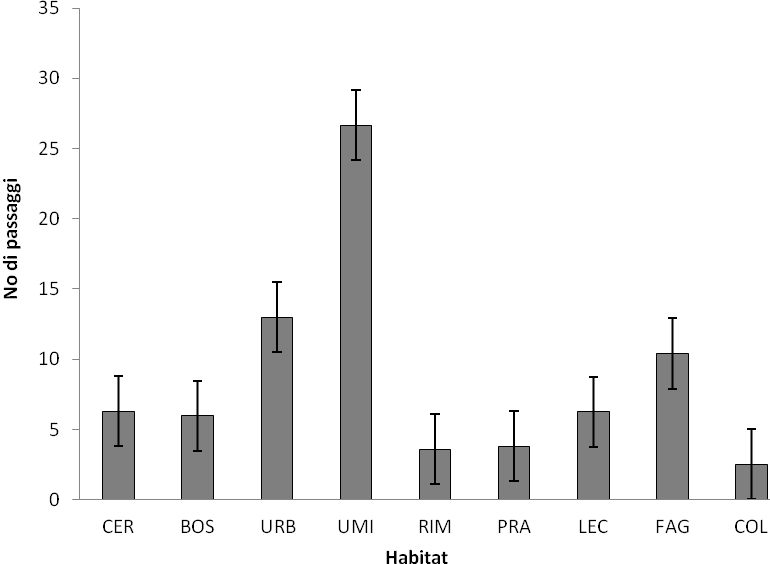
\includegraphics[width=\linewidth]{abstracts/extended_abstracts/P001_Figure1.png}
  \captionof*{figure}{Fig. 1 – Media del numero di passaggi di chirotteri per habitat. La barra di errore rappresenta gli errori standard. CER = Cerrete; BOS = Boschi misti di latifoglie; URB = Aree urbane; UMI = Aree umide; RIM = Rimboschimenti a conifere; PRA = Praterie; LEC = Querceti a leccio; FAG = Faggete; COL = Coltivi.}
\end{Figure}

\subsection*{Modelli di idoneità ambientale}
I modelli di idoneità ambientale applicati nel presente studio sono di tipo induttivo e sono basati su dati di presenza/assenza delle specie sul territorio. La progettazione dei modelli è avvenuta attraverso l’analisi dei dati raccolti sul campo e delle caratteristiche autoecologiche delle specie rilevate, che successivamente sono state correlate con variabili ambientali anche di tipo puntuale, che possono influenzare la presenza delle specie nel territorio oggetto di studio. Le variabili considerate sono: tipologia di habitat e presenza di colonie riproduttive. I modelli sono stati elaborati mediante procedure GIS (\textit{Geographic Information System}), con il \textit{software} ArcGis ver. 9.3 e utilizzando i seguenti dati geografici: la cartografia CORINE Land Cover (IV Livello, 2006) e la Carta Forestale della Basilicata. Gli habitat del parco sono stati classificati e accorpati nelle seguenti categorie: aree umide (laghi e fiumi), rimboschimenti a conifere, querceti a cerro (Cerrete), boschi misti di latifoglie (querceti, ostrieti, carpineti, etc.), coltivi, praterie, boschi di faggio (Faggete), querceti a leccio, aree urbane.

La progettazione ha previsto la restituzione di cartografie, nelle quali il diverso grado di idoneità ambientale è stato suddiviso in 4 categorie:
\begin{compactdesc}
\item[non idoneo]: ambienti che non soddisfano le esigenze ecologiche della specie;
\item[bassa idoneità]: habitat che possono supportare la presenza della specie ma in maniera non stabile nel tempo;
\item[media idoneità]: habitat che possono supportare la presenza stabile della specie, ma che nel complesso non risultano habitat ottimali;
\item[alta idoneità]: habitat ottimali per la presenza della specie.  
\end{compactdesc}
Le cartografie sono state elaborate nel sistema di riferimento UTM WGS 84 – ETRS89 fuso 33N.

\section*{Risultati e discussione}
Nel Parco Nazionale Appennino Lucano Val d’Agri Lagonegrese sono state censite ben 21 specie di chirotteri (Tab.~1, 2).

Complessivamente, mediante campionamento bioacustico sono stati rilevati 885 contatti di chirotteri (Tab.~3), e catturati 61 individui.

I risultati dell’analisi della varianza mostrano che la differenza nella media dei passaggi per gli habitat indagati è statisticamente significativa ($F_{(8,131)}$=4.70, \prob{}=0.00), per cui le tipologie ambientali hanno un effetto significativo sull’attività dei chirotteri. Le risultanze del test \textit{post hoc} di Tukey-Kramer, per un numero ineguale di unità campionarie, mostrano che l’attività differisce significativamente in 7 coppie di habitat (Tab.~4).

Le tipologie ambientali nelle quali è stata riscontrata l’attività più elevata sono le aree umide, seguite dalle aree urbane e gli habitat di tipo forestale, soprattutto le faggete; mentre gli habitat con attività decisamente più ridotta sono i rimboschimenti a conifere ed i coltivi (Fig.~1).
 
Le aree urbane, pur essendo ambienti antropizzati, hanno mostrato un’elevata attività dei chirotteri, specialmente per le specie sinantropiche. La presenza dei lampioni stradali, soprattutto nelle aree periurbane influenza positivamente l’attività ed inoltre, nel territorio del Parco, sono presenti piccoli borghi che spesso risultano strettamente connessi alle matrici naturali del paesaggio e hanno un numero elevato di edifici diroccati importanti per i chirotteri. 

Nel comprensorio del Parco e lungo i confini sono stati censiti 12 rifugi rappresentati prevalentemente da strutture di origine antropica, quali edifici in disuso e una galleria ferroviaria dismessa (Tab.~5). Gli edifici sono tutti ubicati in ambienti poco disturbati e ben integrati nella vegetazione, che nelle zone circostanti è caratterizzata da una copertura variabile da media (50\%) a elevata (80\%). Queste tipologie di rifugi sono utilizzati soprattutto nel periodo estivo e prevalentemente da Rinolofidi e individui maschi. Le colonie riproduttive sono state rilevate esclusivamente nelle cavità di origine naturale ed in particolare nel territorio di San Chirico Raparo (PZ), presso la Grotta di Sant’Angelo al Raparo, che ospita una numerosa colonia polispecifica e nel territorio di Moliterno (PZ), presso la grotta Murgia Sant’Angelo. 

\begin{figure*}[!t] %[!ht]
  \centering\small
  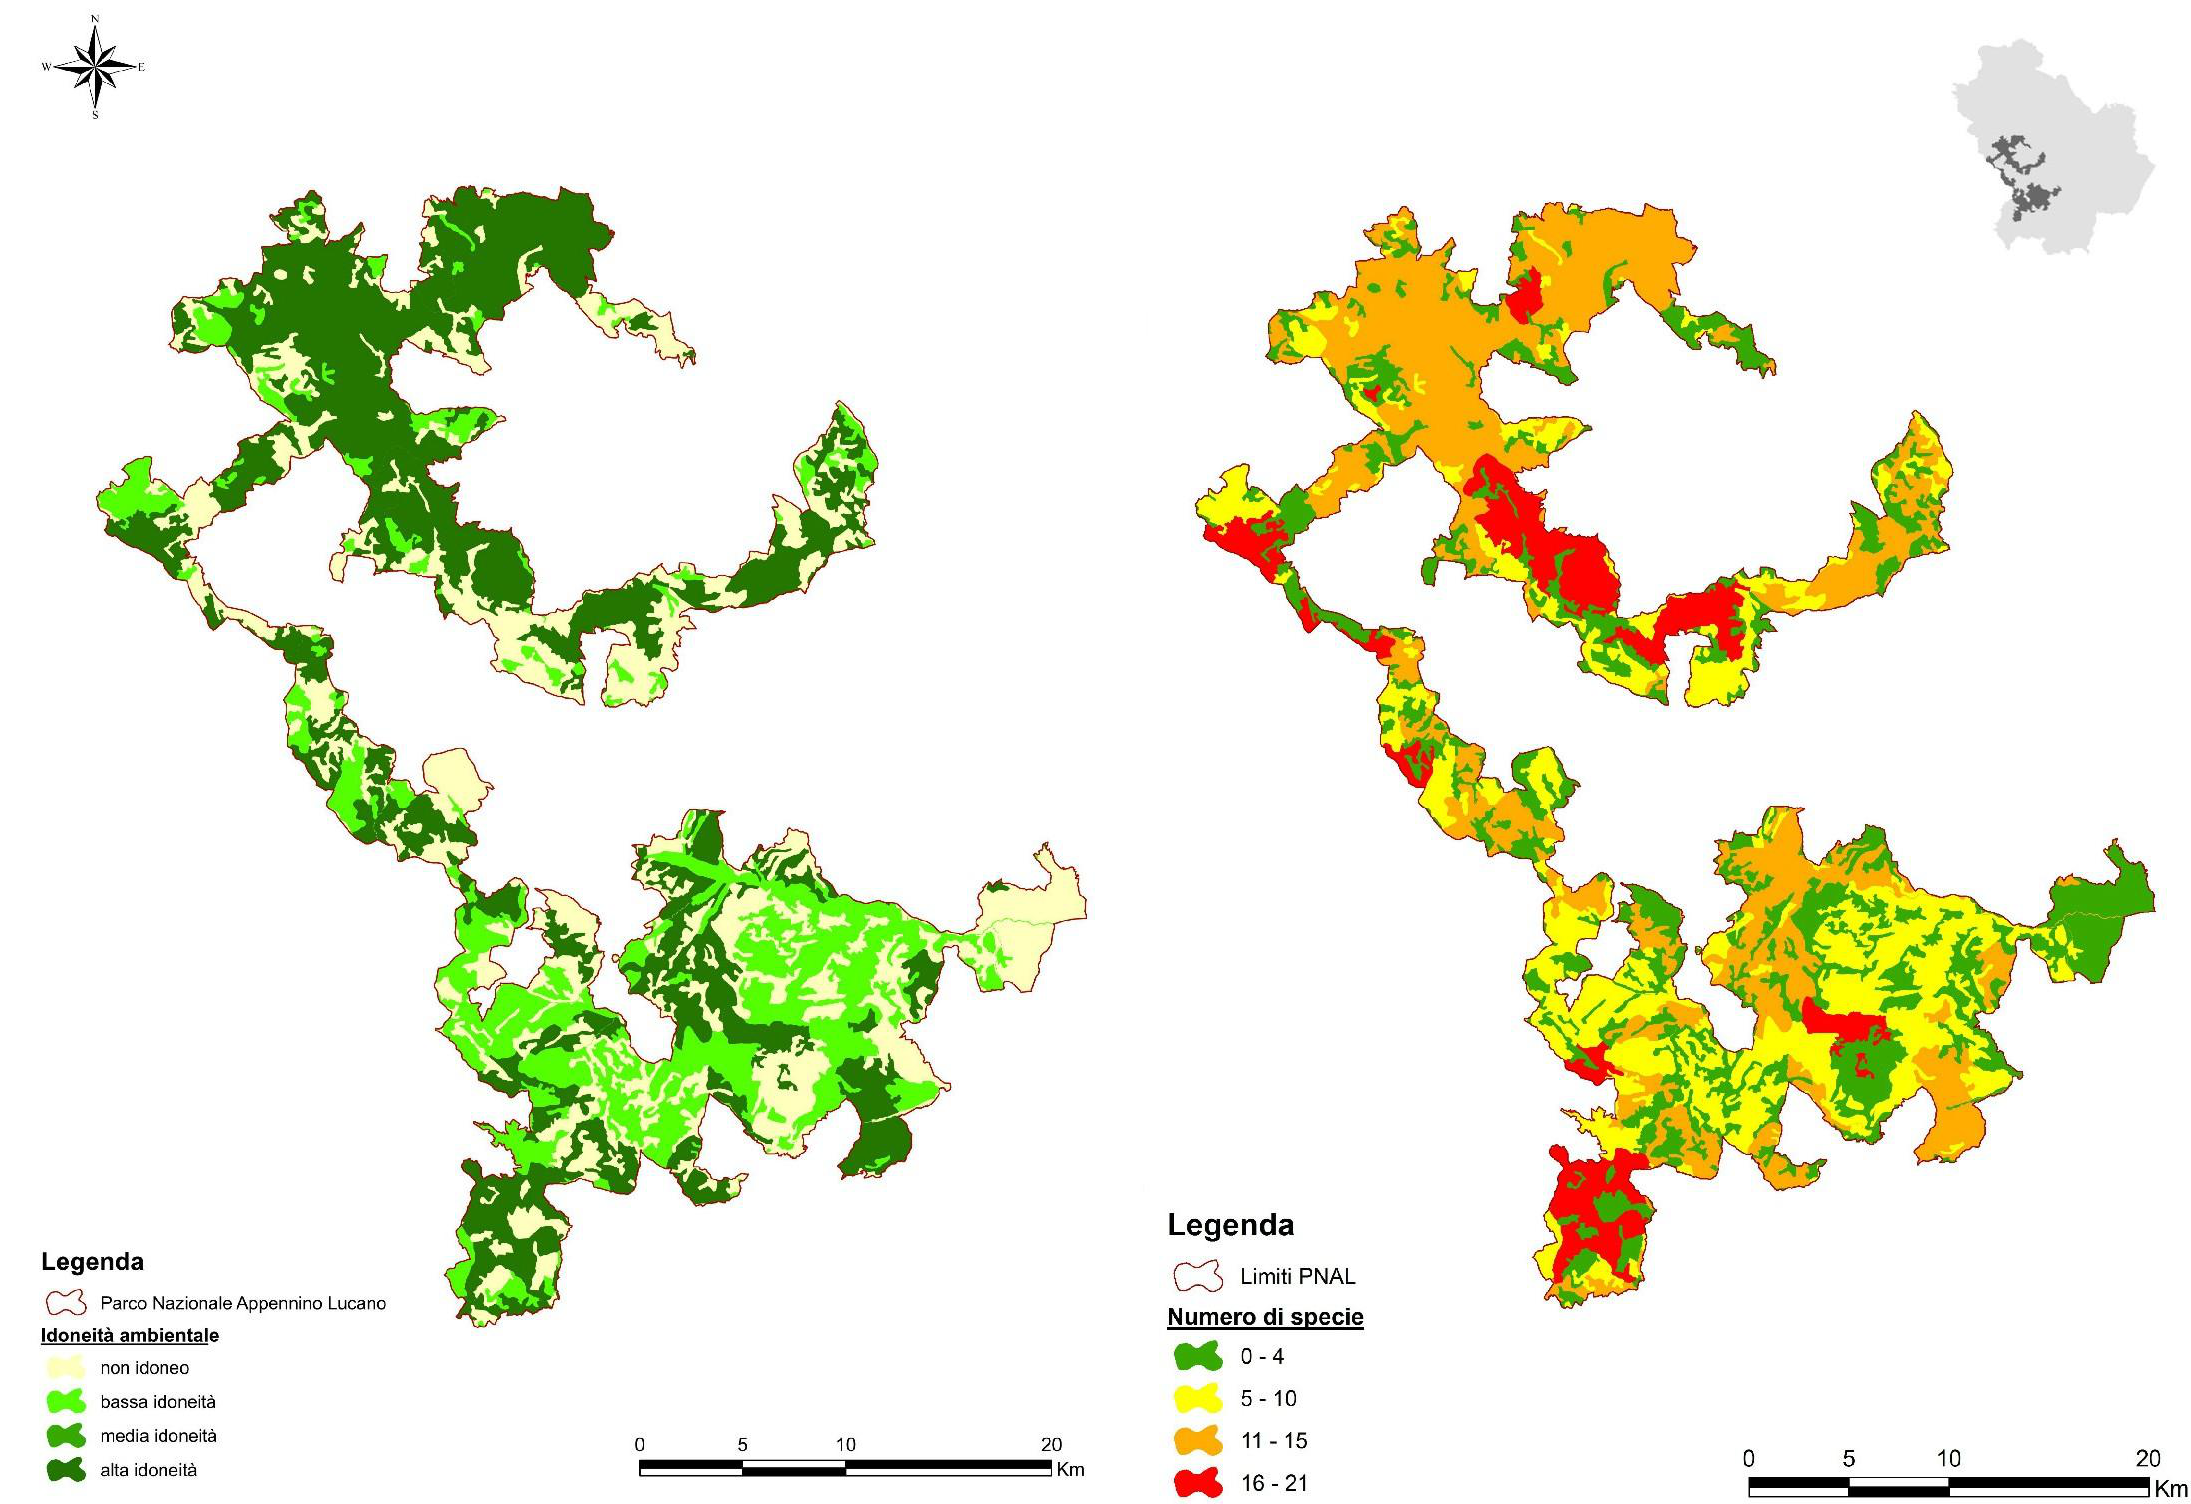
\includegraphics[width=\linewidth]{abstracts/extended_abstracts/P001_Figure2.png}
  \caption*{Fig. 2 - Mappa d’idoneità ambientale per \emph{M. bechsteinii} (a sinistra) e mappa della ricchezza in specie nel PNAL (a destra).}
\end{figure*}

\subsection*{Modelli di idoneità ambientale}
I modelli di idoneità ambientale permettono di integrare e sintetizzare le relazioni specie-ambiente e rappresentano un valido strumento di supporto alle indagini faunistiche conoscitive e ai progetti di conservazione e gestione territoriale (Duprè, 1996; Boitani et al., 2002). 

La progettazione dei modelli di idoneità ambientale ha permesso di confrontare i dati raccolti su gran parte del territorio del Parco, con i dati di letteratura, riguardanti le relazioni specie-habitat. L’analisi sul territorio si è avvalsa dei dati di cattura, relativi ai rifugi e al campionamento bioacustico. Le cartografie risultanti rappresentano la distribuzione potenziale dei chirotteri e la ricchezza di specie (S) nel territorio del Parco (Fig.~2). Gli habitat in cui è stata rilevata una maggiore ricchezza di specie (S), sono in generale gli ambienti forestali, soprattutto i boschi maturi più estesi e meno disturbati da tagli recenti, con alberi vetusti e caratterizzati dalla presenza di aree umide. Gli ambienti in grado di supportare un ridotto numero di specie sono risultati quelli maggiormente antropizzati, rappresentati dalle aree urbane, dai coltivi, soprattutto i seminativi, i rimboschimenti a conifere.

Le aree di maggior pregio per la ricchezza in specie di chirotteri sono per lo più distribuite nel settore settentrionale del Parco (M. Arioso, M. Pierfaone, Serra di Calvello, Monte Volturino, bosco di Rifreddo), dove gli ambienti forestali sono più estesi e presentano un buon grado di eterogeneità ambientale, con popolamenti di varie tipologie e classi di età. Il settore meridionale del Parco (area di Moliterno, Sarconi, San Martino d’Agri) è costituito da ambienti importanti soprattutto per la conservazione dei Rinolofidi, data la presenza di grotte con grandi colonie e di habitat elettivi per l’alimentazione. 

\section*{Conclusioni}
Le informazioni acquisite andranno ad aggiornare significativamente le conoscenze sulla diversità dei chirotteri in Italia meridionale e su scala regionale, che risultano ancora molto lacunose. Alcune specie censite sono tra le più rare nel nostro paese e in Europa, in particolare il Barbastello (\emph{Barbastella barbastellus}) e il Vespertilio di Bechstein (\emph{Myotis bechsteinii}). Importante è anche la presenza di entità criptiche, come \emph{Myotis alcathoe}, che recentemente è stato segnalato nel Parco (De Pasquale et al., 2014) e rappresenta la prima segnalazione della specie per la Basilicata. 

Gli habitat acquatici svolgono un ruolo critico per l’ecologia dei chirotteri, in quanto l’acqua può essere una risorsa limitante che condiziona la loro presenza e l’elevata densità di insetti è un fattore chiave responsabile dell’intensa attività rilevata negli habitat fluviali e lacustri (Barclay, 1991). Nel Parco, le aree umide sono ben rappresentate e molto spesso associate agli habitat forestali, in particolare la diga del Pertusillo, i laghi montani di Piana del lago, nel territorio di Marsico Nuovo (PZ) e di Laudemio, nel territorio di Lagonegro (PZ). 

Molti ambienti forestali risultano minacciati da una cattiva gestione, che ha portato ad una graduale semplificazione strutturale e compositiva dei boschi prevalentemente governati a ceduo, con una ceduazione troppo sostenuta, da turni brevi di taglio, che ha determinato una riduzione del grado di biodiversità e la perdita di rifugi principalmente rappresentati da alberi morti e vetusti.   

Tra i rifugi ipogei censiti, la grotta di Sant’Angelo al Raparo costituisce un sito di importanza biologica per la conservazione dei chirotteri, dato il numero di individui che frequentano la cavità nei diversi periodi dell’anno. Il sito risulta molto accessibile e per questo la tutela può essere compromessa dal disturbo provocato da eventuali visite a scopo didattico, turistico o speleologico, per questo sarà necessaria l’applicazione di misure di conservazione, quali ad esempio il divieto di qualsiasi forma di fruizione della cavità. 

\vskip3mm

\begin{small}
\noindent\textbf{Ringraziamenti}\\
La ricerca è stata finanziata dall’Ente Parco Nazionale dell’Appennino Lucano Val d’Agri Lagonegrese e le attività di cattura sono state autorizzate dal MATTM su parere dell’ISPRA (prot. PNM-2012-0000644). Si ringraziano tutti coloro che hanno collaborato in alcune fasi della ricerca: Dott. Antonio Conte, Sig. Andrea Giudiceandrea, Dott. Remo Bartolomei. 

\vskip3mm

\noindent\textbf{Bibliografia}\\

Agnelli P., Martinoli A., Patriarca E., Russo D., Scaravelli D., Genovesi  P., 2004. Linee Guida per il Monitoraggio dei Chirotteri. Quad. Cons. Natura, 19, Min. Ambiente – INFS

Barclay R.M.R., 1991. Population structure of temperate zone insectivorous bats in relation to foraging behaviour and energy demand. Journal of Animal Ecology 60: 165--178.

Boitani L., Falcucci A, Maiorano L., Montemaggiori A., 2002. Rete Ecologica Nazionale: il ruolo delle aree protette nella conservazione dei vertebrati. Dipartimento B.A.U., Università di Roma ``La Sapienza' , Ministero dell’Ambiente, Dir. per la Conservazione della Natura, Istituto di Ecologia Applicata, Roma.

De Pasquale P.P., Galimberti A., 2014. New records of the Alcathoe bat, \emph{Myotis alcathoe} (Vespertilionidae) for Italy, Barbastella 7, pp. XX ISSN: 1576-9720.

Dietz C., Von Helversen O., 2004. Illustrated identification key to the bats of Europe. Electronic publication, version 1.0, Tübingen, Germany.

Erkert H.G., 1982. Ecological aspects of bat activity rythms. In: Kunz T.H. (Ed.) Ecology of Bats. Plenum Press, New York. 201--242.

Fenton M.B., 1970. A  technique  for monitoring bat activity with results obtained from different environments in southern Ontario. Canadian Journal of Zoology, 48: 847--851.
 
Galimberti A., Spada M., Russo D., Mucedda M., Agnelli P., et al., 2012. Integrated Operational Taxonomic Units (IOTUs) in Echolocating bats: a bridge with Molecular  and Traditional Taxonomy. PLoS ONE  7(6): e40122. \url{doi:10.1371/journal.pone.0040122}
  
Grindal  S.D.,  Collard T.S., Brigham R.M.,  Barclay R.M., 1992. The influence of precipitation on  reproduction by  \emph{Myotis} Bats in British Columbia. American Midland Naturalist 128: 339--344.

Kramer A.C.Y., 1956). Extention of multiple range tests to group means with unequal numbers of replications. Biometrics 12: 307--310.

Kunz T.H., Kurta A., 1988. Capture methods and holding devices. In: Kunz T.H. (Ed.) Ecological and Behavioral Methods for the Study of Bats. Smithsonian Institution Press, Washington, DC. 1--29.
 
Russo D., Jones G., 2000. The two cryptic species of \emph{Pipistrellus pipistrellus} (Chiroptera: Vespertilionidae) occur in Italy: evidence from echolocation and social calls. Mammalia 64: 187--197.

Russo D., Jones G., 2002. Identification  of  twenty-two bat species  (Mammalia: Chiroptera)  from Italy by analysis  of  time-expanded  recordings  of echolocation calls. Journal of Zoology (London)  258: 91--103.
 
Tukey J.W., 1949. Comparing individual means in the analysis of variance. Biometrics 5: 99.

Whitloch M.C., Schluter D., 2010. Analisi statistica dei dati biologici. Zanichelli.

Worthington-Wilmer J., Barratt E.M., 1996. A nonlethal method of tissue sampling for genetic studies of chiropterans. Bat Research News 37: 1-–3. 

\end{small}

\end{multicols}
% % EOF % %